%%%%%%%%%%%%%%%%%%%%%%%%%%%%%%%%%%%%%%%%%%%%%%%%%%%%%%%%%%%%
%%  This Beamer template was created by Cameron Bracken.
%%  Anyone can freely use or modify it for any purpose
%%  without attribution.
%%
%%  Last Modified: January 9, 2009
%%

\documentclass[xcolor=x11names,compress, graphics]{beamer}

%% General document %%%%%%%%%%%%%%%%%%%%%%%%%%%%%%%%%%
\usepackage{graphicx}
\usepackage{tikz}
\usetikzlibrary{decorations.fractals}
%%%%%%%%%%%%%%%%%%%%%%%%%%%%%%%%%%%%%%%%%%%%%%%%%%%%%%
\usepackage{movie15}
\usepackage{float}
\usepackage{subfig}
\usepackage{amsmath}
\usepackage{amsfonts}
\usepackage{mathrsfs}
\usepackage{mathtools}

\usepackage{algorithm, algorithmic}

%% Beamer Layout %%%%%%%%%%%%%%%%%%%%%%%%%%%%%%%%%%
\useoutertheme[subsection=false,shadow]{miniframes}
\useinnertheme{default}
\usefonttheme{serif}
\usepackage{palatino}

\setbeamerfont{title like}{shape=\scshape}
\setbeamerfont{frametitle}{shape=\scshape}

\setbeamercolor*{lower separation line head}{bg=DeepSkyBlue4} 
\setbeamercolor*{normal text}{fg=black,bg=white} 
\setbeamercolor*{alerted text}{fg=red} 
\setbeamercolor*{example text}{fg=black} 
\setbeamercolor*{structure}{fg=black} 
 
\setbeamercolor*{palette tertiary}{fg=black,bg=black!10} 
\setbeamercolor*{palette secondary}{fg=black,bg=black!10}
\setbeamercolor*{palette quaternary}{fg=black,bg=black!10} 

%% Set the background and font color of the blocks 
\setbeamercolor{block title}{bg=DeepSkyBlue4,fg=white}

%% Set the type of the blocks
\setbeamertemplate{blocks}[shadow=true]

\newcommand{\topline}{%
  \tikz[remember picture,overlay] {%
    \draw[DeepSkyBlue4] ([yshift=-1.5cm, xshift = 1cm]current page.north west)
             -- ([yshift=-1.5cm,xshift=\paperwidth-1cm]current page.north west);}}
             
\setbeamertemplate{section in toc}[sections numbered]           

\renewcommand{\(}{\begin{columns}}
\renewcommand{\)}{\end{columns}}
\newcommand{\<}[1]{\begin{column}{#1}}
\renewcommand{\>}{\end{column}}

\usepackage[skip=10pt,font=scriptsize]{caption}
\captionsetup[figure]{labelformat=empty}

\DeclarePairedDelimiter\floor{\lfloor}{\rfloor}

\makeatother
\setbeamertemplate{footline}
{
  \leavevmode%
  \hbox{%
  \begin{beamercolorbox}[wd=.4\paperwidth,ht=2.25ex,dp=1ex,center]{author in head/foot}%
    \usebeamerfont{author in head/foot}\insertshortauthor
  \end{beamercolorbox}%
  \begin{beamercolorbox}[wd=.6\paperwidth,ht=2.25ex,dp=1ex,center]{title in head/foot}%
    \usebeamerfont{title in head/foot}\insertshorttitle\hspace*{3em}
    \insertframenumber{} / \inserttotalframenumber\hspace*{1ex}
  \end{beamercolorbox}}%
  \vskip0pt%
}
\makeatletter
%%%%%%%%%%%%%%%%%%%%%%%%%%%%%%%%%%%%%%%%%%%%%%%%%%

\title{\scshape \textbf{Asymptotic Analysis}}
\author{\scriptsize\scshape Angel No\'e Mart\'inez Gonz\'alez}


\begin{document}

% The title page
\begin{frame}
\setcounter{framenumber}{1}
\titlepage
\scriptsize

\end{frame}
%===============


\section[\scshape Motivation]{\scshape Motivation}
\begin{frame}[allowframebreaks]{Motivation}
\topline

{\scshape Why analysing algorithms? }
\begin{itemize}
	\item Predict resources an algorithm requires: memory, bandwidth, etc.
	\item Identify the most efficient algorithm between several others.
	\item Improve efficiency of an existing algorithm.
	\item For fun!
\end{itemize}


\framebreak
\topline

{\scshape How do we analyse algorithms? }
\begin{itemize}
	\item Model of the technology: RAM, PC.
	\item Mathematical tools or analysis (not so damn complicated!).
	\item Asymptotic analysis, i.e. when n goes to infinity.
\end{itemize}
\vspace{.5cm}
{\scshape We only consider two important factors: }
\begin{enumerate}
	\item Input size $n \in \mathbb{N}$. Assume $n$ large. 
	\item Running time $T(n)$: number of primitive operations or "steps" executed for the given input.
\end{enumerate}


\end{frame}

\section[\scshape Starting]{\scshape Getting Started}
\begin{frame}[allowframebreaks]{Getting started: the sorting problem}
\topline

Given a sequence of numbers $A=[a_1,a_2,...,a_n]$ as input, generate a permutation of the input such that $a'_1 \leq a'_n \leq ... \leq a'_n $
\\

\begin{figure}
    \begin{center}
        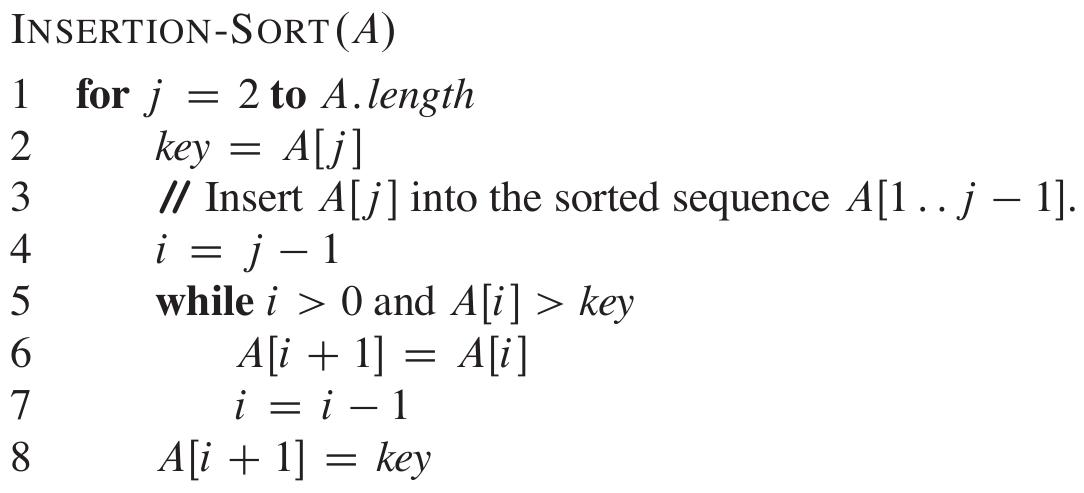
\includegraphics[width=10cm]{Figures/InsertionSort.jpeg}
    \end{center}
\end{figure}


\framebreak
\topline
{\scshape\Large Analysis}
\vspace{1cm}
\begin{itemize}
	\item Assume each instruction has a constant given time.
	\item Look how many times the instruction is executed.
	\item Take the product of the two above.
	\item The total running time is the sum of all instructions running times.
\end{itemize}


\framebreak
\topline
\begin{figure}
    \begin{center}
        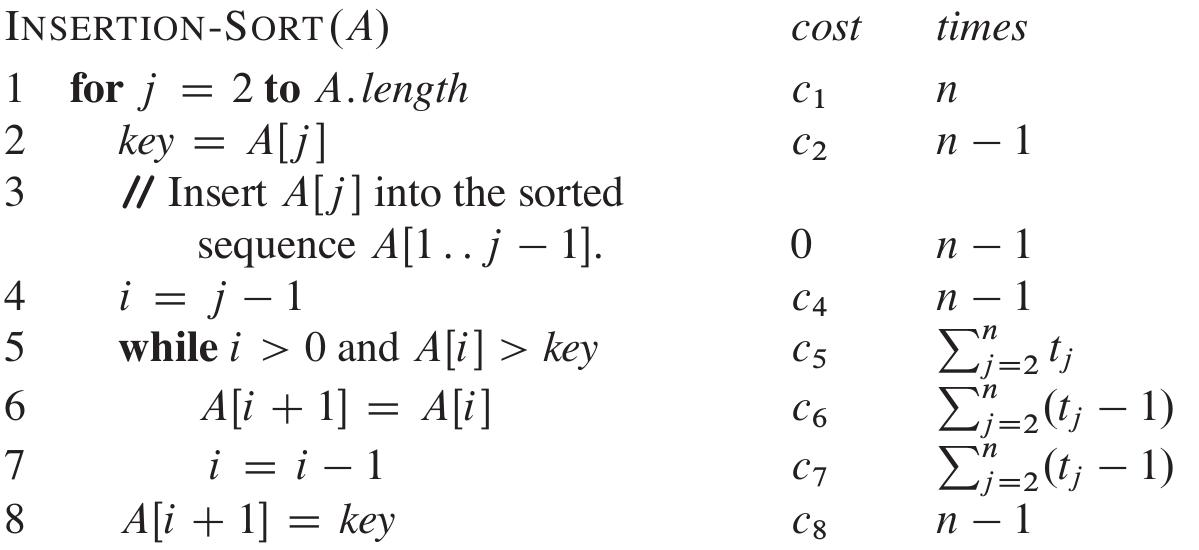
\includegraphics[width=11cm]{Figures/InsertionSortAnalysis.jpeg}
    \end{center}
\end{figure}



\framebreak
\topline
The running time $T(n)$ for insertion sort is

{\small
$$
T(n) = c_1n + c_2(n-1) + c_4(n-1) + c_5\sum_{j=2}^nt_j + c_6\sum_{j=2}^n(t_j-1) + c_7\sum_{j=2}^n(t_j-1) + c_8(n-1)
$$
}

Solving recurrences

{\scriptsize
$$
T(n) = \left( c_5+c_6+c_7 \right) \frac{1}{2}n^2 + \left(c_1 + c_2 + c_4 + \frac{c_5}{2} - \frac{c_6}{2} - \frac{c_7}{2} + c_8 \right)n -\left( c_2 + c_5 + c_5 + c_8 \right)
$$
}

Which can be represented as

{\scriptsize
$$
T(n) = a\cdot n^2 + b\cdot n + c
$$
}

\end{frame}


\section[\scshape Cases]{\scshape Worst and Average Case}
\begin{frame}[allowframebreaks]{Worst and Average Case}
\topline

{\scshape\Large Average case }
\vspace{.5cm}

\begin{enumerate}
    \item Analyse the average running time of an algorithm.
    \item Requires domain knowledge.
    \item Analyse for specific inputs.
    \item Bit more complex to analyse input distributions, etc.
\end{enumerate}

\framebreak
\topline

{\scshape\Large Worst case }
\vspace{.5cm}

\begin{enumerate}
    \item Upper bounds on the running time of an algorithm.
    \item Worst case occurs fairly often!
    \item Analysis hold for every input.
    \item Useful for general purpose algorithms.
    \item Mathematically more tractable.
\end{enumerate}

We will focus mainly in the worst case analysis.

\end{frame}

\section[\scshape Big Oh]{\scshape Big Oh Notation}
\begin{frame}[allowframebreaks]{Big $O$ Notation}
\topline
Denotes asymptotic upper bound. For a given function $g(n)$, we denote by $O(g(n))$ the set of functions

\vspace{.5cm}

\begin{eqnarray*}
O(g(n)) & = &\{ f(n): \text{There exists positive constans $c$ and $n_0$}\\
& & \text{such that $0 \leq f(n) \leq cg(n)$ for all $n > n_0$} \}
\end{eqnarray*}

\vspace{.5cm}

We say that $T(n)=O(g(n))$ when $T(n)$ is bounded above for a constant multiple of $g(n)$.

\framebreak
\topline

{\scshape\Large In other words }

\vspace{.5cm}

\begin{minipage}{5cm}
\begin{figure}
	\begin{center}
		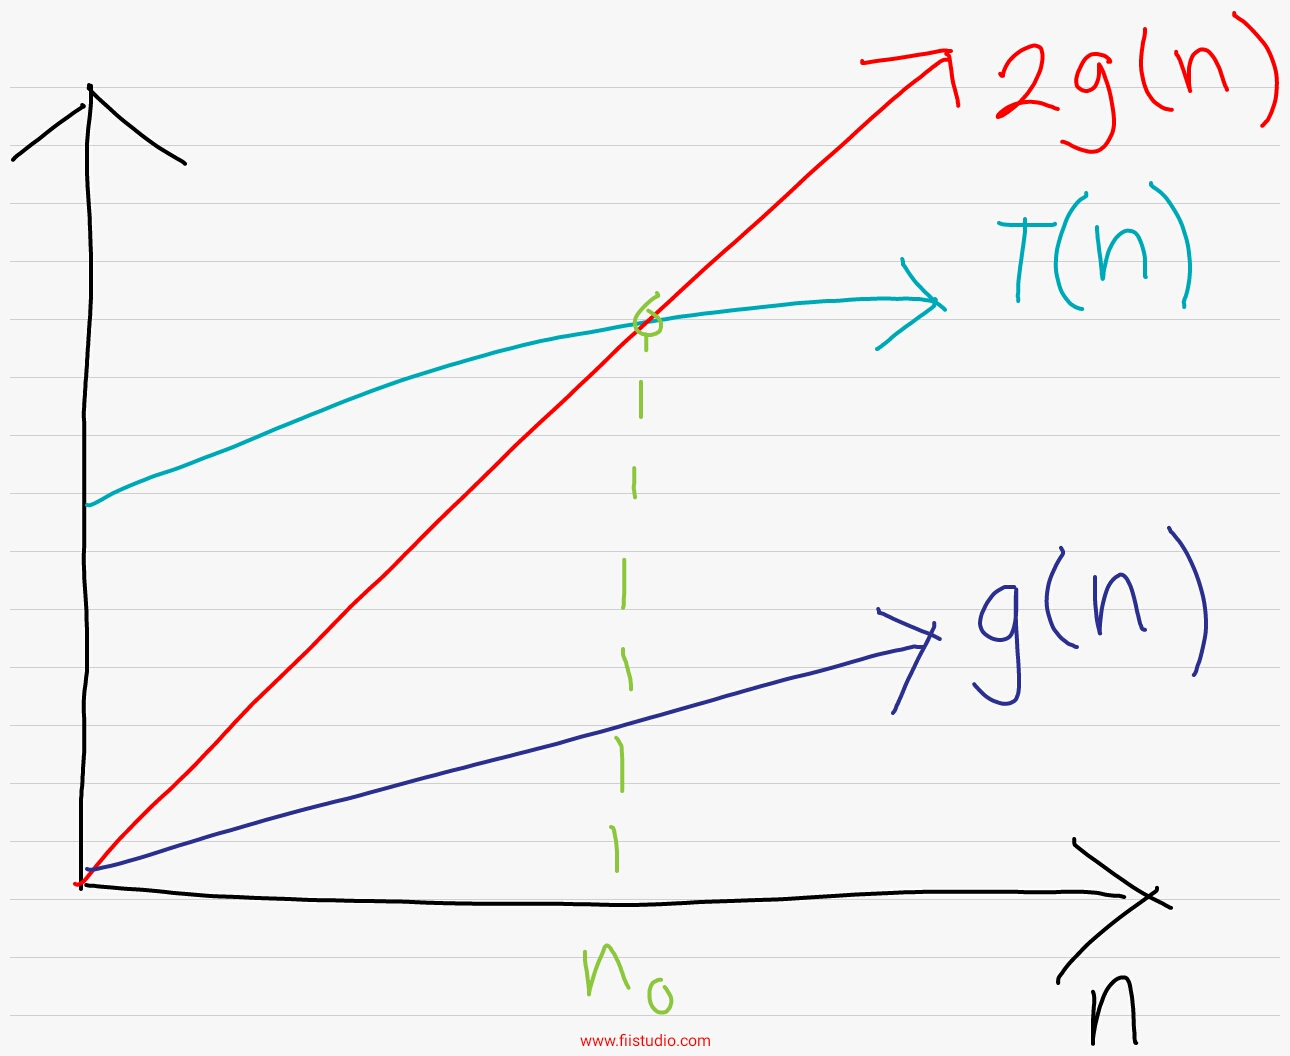
\includegraphics[width=5cm]{Figures/O_n.jpg}
	\end{center}
\end{figure}
\end{minipage}\ \ 
\begin{minipage}{5cm}
$T(n)=O(g(n))$ if and only if exist $c,n_0>0$ such that
$$
T(n) \leq cg(n)
$$
for all $n\geq n_0$ and $c,n_0$ independent of $n$.
\end{minipage}

\end{frame}

\section[\scshape Comparing]{\scshape Merge Sort}
\begin{frame}[allowframebreaks]{How to compare?}
\topline

{\scshape\Large Divide and Conquer Intro: Merge Sort}

\begin{minipage}{5cm}

\captionof*{algorithm}{}{{\scshape merge-sort}($A, p, r$)}
\begin{algorithmic}[1]
\IF{$p<r$}
	\STATE $q = \floor*{(p+r)/2}$
	\STATE {\scshape merge-sort}($A, p, q$)
	\STATE {\scshape merge-sort}($A, q, r$)
	\STATE {\scshape merge}($A, p, q, r$)
\ENDIF
\end{algorithmic}

\end{minipage}\ \ 
\begin{minipage}{5cm}

\captionof*{algorithm}{}{{\scshape merge}($A, p, q, r$)}
\begin{algorithmic}[1]
\STATE $B=1^{st}$ part of array.
\STATE $C=2^{nd}$ part of array.
\STATE $i=1,j=1$
\FOR{$k=1$ to $n$}
	\IF{$B[i]<C[j]$}
		\STATE $A[k]=B[i]$
%		\STATE $i++$
	\ELSE
		\STATE $A[k]=C[j]$
%		\STATE $j++$
	\ENDIF
\ENDFOR
\end{algorithmic}

\end{minipage}

\framebreak
\topline

{\scshape\Large An Example tree}

\begin{figure}
	\begin{center}
		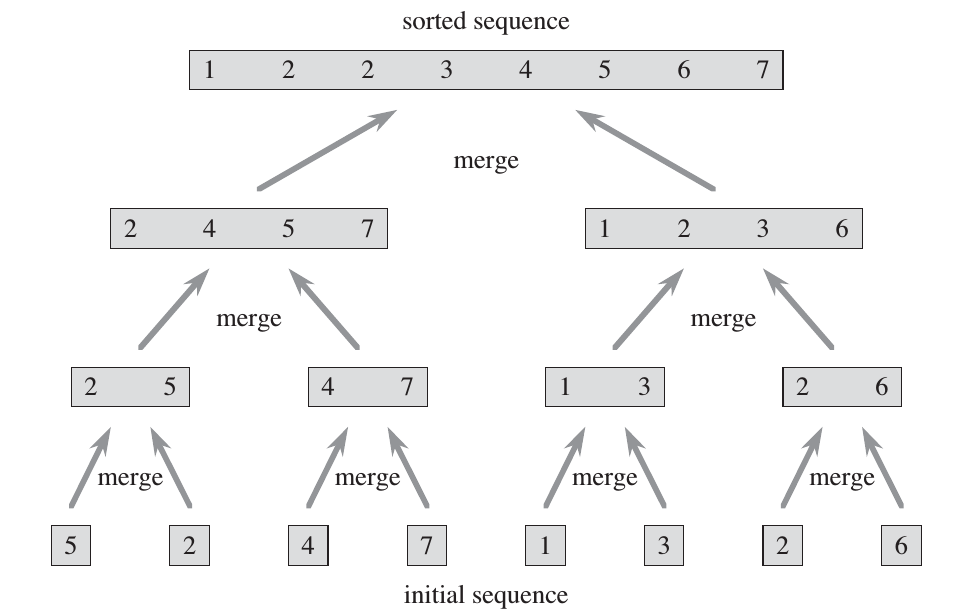
\includegraphics[width=8cm]{Figures/mergeSortTree.png}
	\end{center}
\end{figure}

At each level $j=0,1,...,log_2(n)$, there are $2^j$ subproblems of size $n/2^j$.


\framebreak
\topline

Now let's say that subroutine {\scshape merge}($A,p,q,r$) takes $m\cdot x$, with $x=n/2^j$ and a constant $m$. Then for each level {\scshape merge}($A,p,q,r$) costs

$$
2^j\cdot m\cdot \frac{n}{2^j}=m\cdot n
$$

Then, the running time of {\scshape merge-sort}($A,p,r$) is

$$
T(n) = m\cdot n\cdot log_2(n) + m\cdot n
$$

Finally we get that $O(m\cdot n\cdot log_2(n) + m\cdot n)$ is better than $O(a\cdot n^2 + b\cdot n + c)$.

\end{frame}

\section[\scshape Guiding]{\scshape Guiding Principles}
\begin{frame}[allowframebreaks]{Guiding Principles}
\topline
{\scshape\Large When analysing algorithms}
\vspace{.5cm}
\begin{itemize}
	\item Don't pay attention in constant factors: dependent on architecture, compiler, programmer, etc.
	\item Consider each input as equally likely.
	\item Assume very large input problems, i.e. large $n$.	
	\item Use the abstraction power of asymptotic analysis: $O(n\cdot log_2(n))$ is better than $O(n^2 )$.
\end{itemize}

\framebreak
\topline

{\scshape\Large Sometimes look deeper!}

\begin{minipage}{5cm}

\begin{figure}
	\begin{center}
		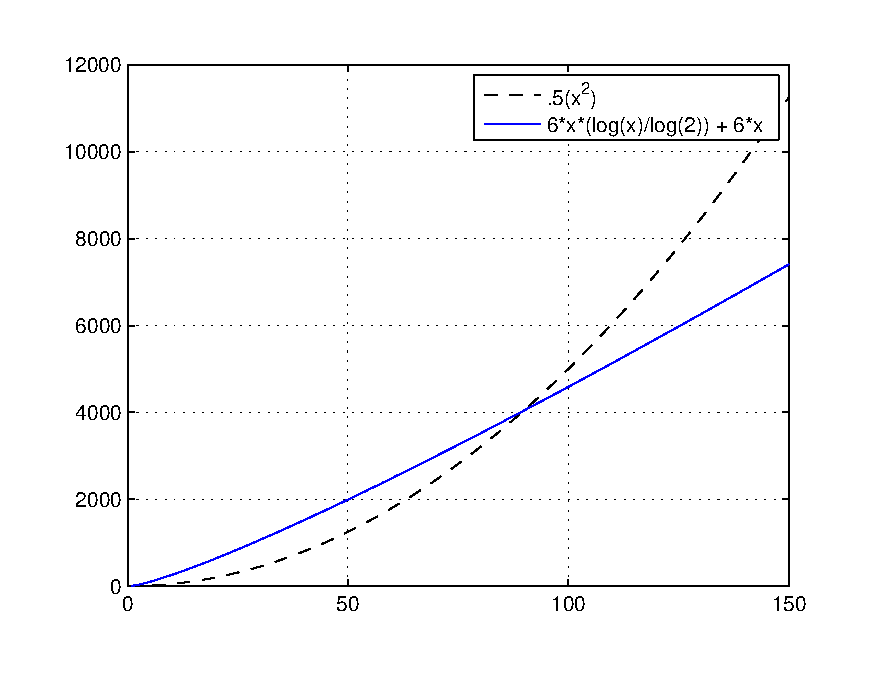
\includegraphics[width=6cm]{Figures/betterInsertion.eps}
	\end{center}
\end{figure}

\end{minipage}\ \ \ \ \ 
\begin{minipage}{5cm}

\begin{figure}
	\begin{center}
		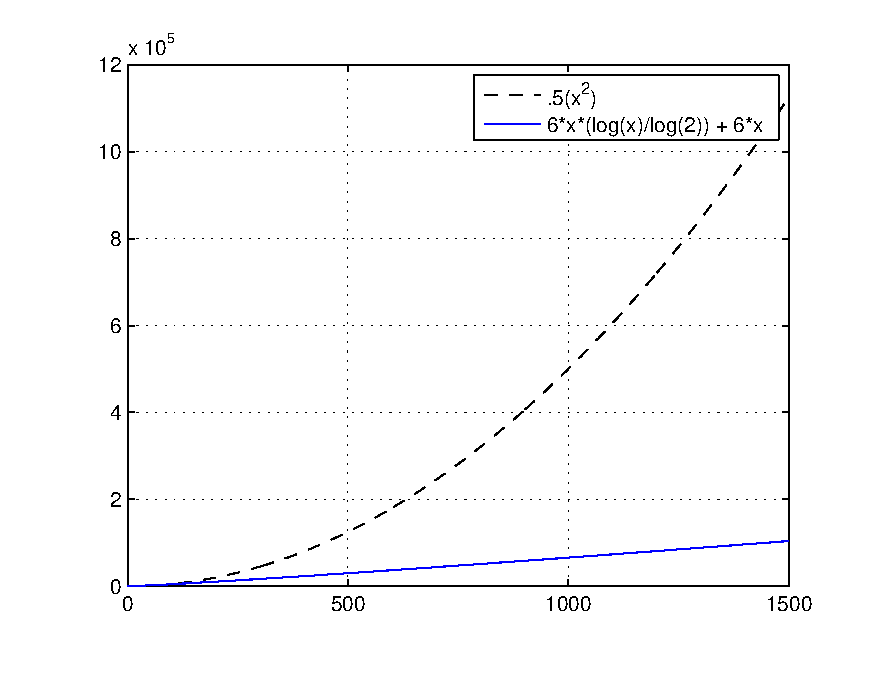
\includegraphics[width=6cm]{Figures/betterMerge.eps}
	\end{center}
\end{figure}

\end{minipage}

\framebreak
\topline 

\begin{figure}
	\begin{center}
		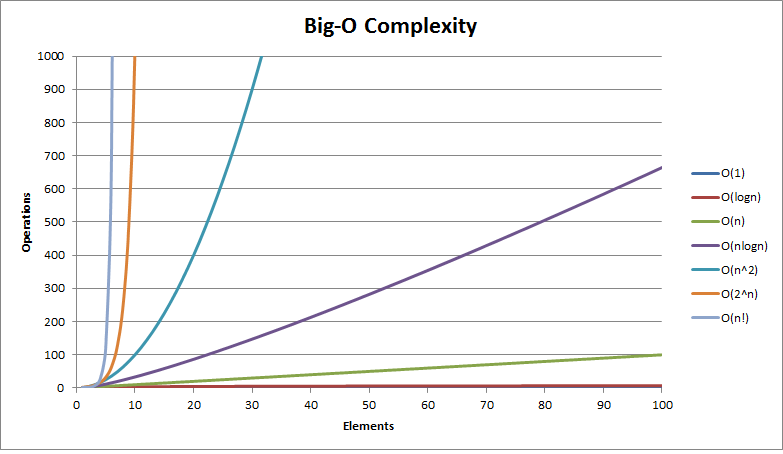
\includegraphics[width=10cm]{Figures/big-o-complexity.png}
	\end{center}
\end{figure}

From \emph{http://bigocheatsheet.com/}

\end{frame}

\section[\scshape Big $\Omega$ and $\Theta$]{Big $\Omega$ and $\Theta$}
\begin{frame}[allowframebreaks]{Big $\Omega$ and $\Theta$}

{\scshape\Large Big $\Omega$}: provides an asymptotic lower bound.

\vspace{.5cm}

\begin{minipage}{5cm}
\begin{figure}
	\begin{center}
		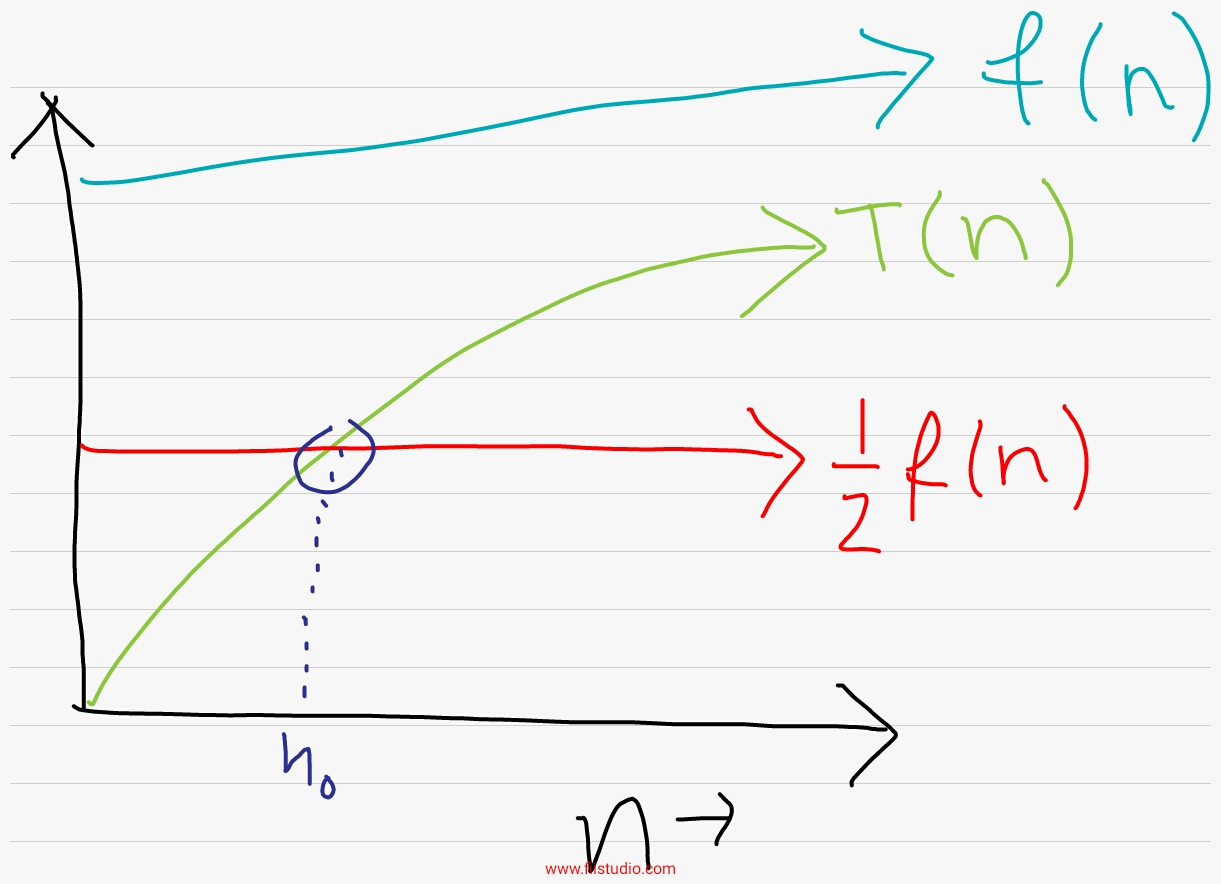
\includegraphics[width=5cm]{Figures/Omega_n.jpg}
	\end{center}
\end{figure}
\end{minipage}\ \ 
\begin{minipage}{5cm}

$T(n)=\Omega(f(n))$ if and only if exist constants $c$ and $n_0$ such that

$$
T(n) \geq cf(n)
$$

For all $n\geq n_0$.

\end{minipage}

\framebreak
\topline

{\scshape\Large Big $\Theta$}: provides asymptotic ranges.

\vspace{.5cm}

\begin{minipage}{5cm}
\begin{figure}
	\begin{center}
		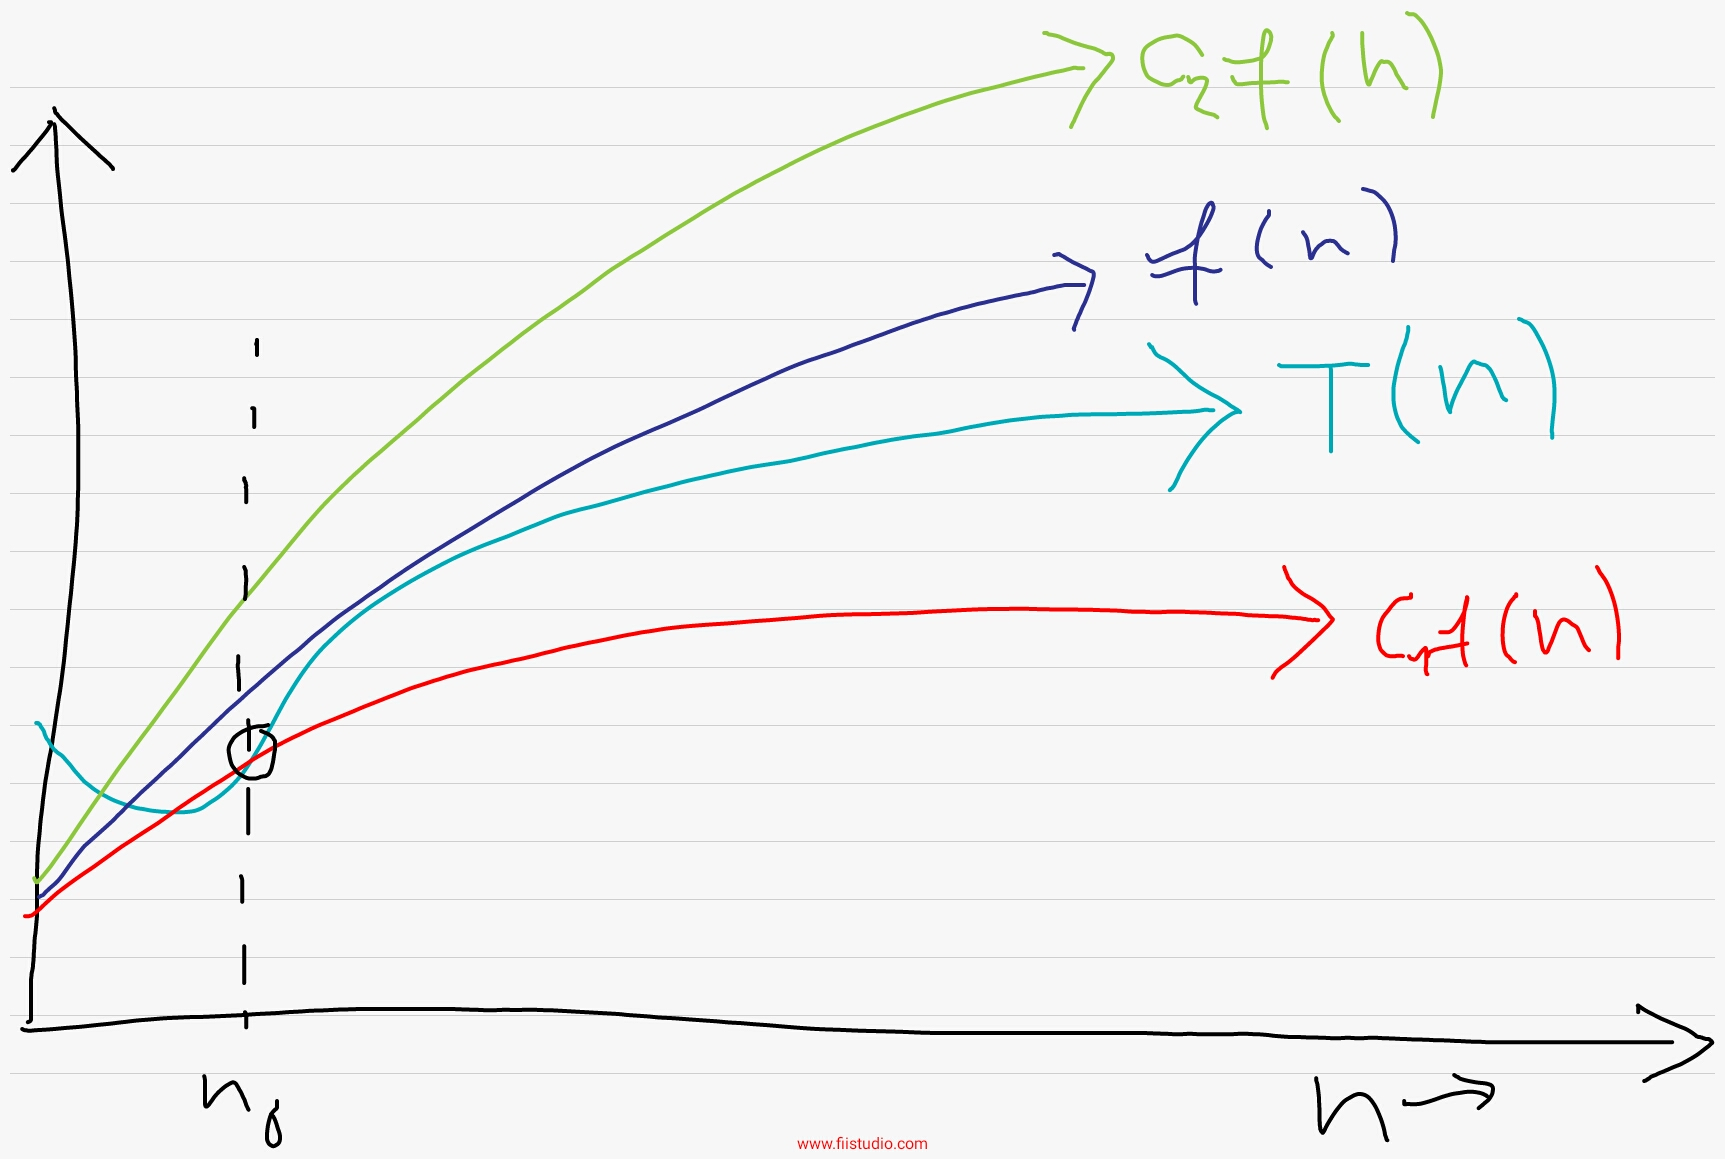
\includegraphics[width=5cm]{Figures/Theta_n.jpg}
	\end{center}
\end{figure}
\end{minipage}\ \ 
\begin{minipage}{5cm}

$T(n)=\Theta(f(n))$ if and only if exist constants $c_1$, $c_2$ and $n_0$ such that

$$
c_1f(n) \leq T(n) \leq c_2f(n)
$$

For all $n\geq n_0$.

\end{minipage}

\vspace{.5cm}

Note $T(n)=\Theta(f(n))$ implies that $T(n)=O(f(n))$ and $T(n)=\Omega(f(n))$.
\end{frame}

\section[\scshape Little $\omega$ and $\theta$]{Little $\omega$ and $\theta$}
\begin{frame}[allowframebreaks]{Little $o$, $\omega$ and $\theta$}
\topline

Little $o$, $\omega$ and $\theta$ lose tightness in the bounds.

\vspace{.5cm}

\begin{enumerate}
	\item[$o(g(n))$] $=\{f(n):\text{ $\exists$ $c,n_0 > 0$ $|$ $ 0 \leq f(n) < cg(n)$  $\forall$  $n\geq n_0$ } \}$
	\item[$\omega(g(n))$] $=\{f(n):\text{ $\exists$ $c,n_0 > 0$ $|$ $ 0 \leq cg(n) < f(n)$  $\forall$  $n\geq n_0$ } \}$
	\item[$\theta(g(n))$] $=\{f(n):\text{ $\exists$ $c_1,c_2,n_0 > 0$ $|$ $ c_1g(n) < f(n) < c_2g(n)$  $\forall$  $n\geq n_0$ } \}$
\end{enumerate}

\end{frame}



\end{document}